\documentclass{deliverablereport}
\usepackage[style=alphabetic,backend=bibtex]{biblatex}
\addbibresource{../../lib/kbibs/kwarcpubs.bib}
\addbibresource{../../lib/kbibs/extpubs.bib}
\addbibresource{../../lib/kbibs/kwarccrossrefs.bib}
\addbibresource{../../lib/kbibs/extcrossrefs.bib}
\addbibresource{../../lib/deliverables.bib}
\addbibresource{local.bib}
%\usepackage{local}
\usepackage[show]{ed}
\usepackage{stex-logo}
\usepackage{rotating}
\usepackage{tikzinput}
\usetikzlibrary{fit}
\title{Curated Math-in-the-Middle Ontology and Alignments for GAP/SAGE/LMFDB}
\def\shorttitle{Curated MitM Ontology/Alignments}

\deliverable{dksbases}{lfmverif}
\deliverydate{1/07/2018}
\duedate{1/09/2018}

\author{John Cremona}
\author{Dennis M\"uller}
\author{Michael Kohlhase}
\author{Markus Pfeiffer}
\author{Florian Rabe}
\author{Nicolas M. Thiéry}
\author{Tom Wiesing}

\begin{document}
\maketitle
\begin{abstract}
  Work Package WP6 develops a novel, foundational, knowledge-based framework for
  interfacing existing open source mathematical software systems and knowledge bases into
  a mathematical VRE, where systems can delegate functionalities among each other
  seamlessly without losing semantics.

  The overall Math-in-the-Middle (MitM) Framework developed in WP6 over the last three
  years is described in D6.5; this Report complements it by describing the curated
  contents Math-in-the-Middle (MitM) Ontology which serves as a reference and pivotal
  point for translations between the various input languages of mathematical software
  systems and knowledge bases.

  In a nutshell, the MitM Ontology describes the mathematical objects, concepts, and their
  relations in a general, system-agnostic way in an OMDoc/MMT theory graph while the
  mathematical systems export API theories that describe the system interface language in
  terms of types, classes, constructors, and functions -- again in OMDoc/MMT. These two
  levels of descriptions are linked by OMDoc/MMT alignments that allow the translation of
  expressions between systems.
\end{abstract}
%\newpage\strut\githubissuedescription
\tableofcontents\newpage

\section{Introduction}
The Math-in-the-Middle (MitM) Ontology is developed in the OpenDreamKit project as a
central information resource for the Math-in-the-Middle (MitM) approach to flexible and
knowledge-based integration of mathematical software systems. It serves as a reference and
pivotal point for translations between the various input languages of mathematical
software systems. This integration and interoperability has been described
in~\cite{DehKohKon:iop16,WieKohRab:vtuimkb17,KohMuePfe:kbimss17} and -- in great detail --
in \cite{ODK-D6.5}. In a nutshell, the MitM Ontology describes the mathematical objects,
concepts, and their relations in a general, system-agnostic way in an OMDoc/MMT theory
graph while the mathematical systems export API theories that describe the system
interface language in terms of types, classes, constructors, and functions -- again in
OMDoc/MMT. These two levels of descriptions are linked by OMDoc/MMT
alignments~\cite{MueGauKal:cacfms17} that allow the translation of expressions in the
interface language of system $A$ into the MitM-induced language, and from there to the
interface language of system $B$~\cite{MueRoYuRa:abtafs17}.

The Math-in-the-Middle Ontology is hosted on the MathHub.info system~\cite{IanJucKoh:sdm14,MathHub:on}, the sources can be obtained from \url{http://gl.mathhub.info}.
As the MathHub front-end is currently undergoing major re-write\footnote{The old MathHub interface was based on Drupal, which led to major system vulnerabilities and therefore maintenance hassles, because Drupal was targeted by hackers.
  We are currently working on a docker-based orchestration of services with a React.JS based front-end in the general spirit of the OpenDreamKit VRE toolkit; see \url{https://github.com/MathHubInfo/}.
  The new system can be accessed at \url{http://new.mathhub.info}.} we will reference the MitM ontology by its sources -- the semantically enhanced user interface can be accessed via the same URLs without the \url{gl.} part.

The development consists of four parts:
\begin{compactenum}[\em i\rm)]
\item The \textbf{MitM ontology} which has the formalization of mathematical background theories
  which expresses the knowledge in terms of mathematical concepts found in the
  mathematical literature, without concern -- and thus abstracting from -- for system
  requirements.
\item The \textbf{SMGloM Glossary} which has a human-oriented -- and thus informal --, but
  semantically structured versions of the same content, and can therefore act as a
  human-readable documentation.
\item \textbf{System API theories for the OpenDreamKit Systems and mathematical data bases}, these
  express the system-specific instances of the mathematical concepts, constructors,
  procedures, and types that make up the input/output language of the respective systems.
\item The \textbf{Alignments} between the OpenDreamKit System API theories and the MitM ontology. 
\end{compactenum}
We will discuss all four parts separately below, and conclude with a self assessment of the MitM at this stage.

\section{The MitM Ontology}\label{sec:mitmonto}
%% types
\newcommand{\fold}[2]{\let\@tmpop=\relax\@for\@I:=#2\do{\@tmpop\@I\let\@tmpop=#1}}
\newcommand{\record}[1]{\{\fold{,}{#1}\}}
\newcommand{\union}[1]{[\fold{,}{#1}]}
\newcommand{\sq}{\subseteq}

In this section, we describe the parts of the MitM ontology, which is a formal development in the MMT system.
The formalizations can be found at \url{https://gl.mathhub.info/MitM/}.
That location also contains various other archives in the \href{https://gl.mathhub.info/MitM/}{\texttt{MitM} library}, which are experiments, where the MitM ontology has been picked up by other projects.

The MitM ontology consists of two parts: the \textbf{MitM Foundation} which provides the logical language in which the mathematical domains in the MitM ontology can be described, and the \textbf{MitM Core}, which consists of the knowledge about these domains represented in the MitM foundation.

\subsection{The MitM Foundation}\label{sec:foundation}

The MitM foundation provides the type system and logic for the MitM ontology, i.e., the basic representational infrastructure used in the MitM ontology.
It is developed in the archive  \href{https://gl.mathhub.info/MitM/Foundation}{\texttt{Foundation}} (4 files, 539 LoF (lines
of formalization), 103 commits).

\paragraph{Types \& Expressions}
While the logic is relatively straightforward, the standardization of the type system was very difficult because mathematics requires a rich, open-ended type system, yet concrete implementations must stay as simple as possible.
After surveying the OpenDreamKit systems, we developed the types described in Appendix~\ref{app:types}.
These types come with a set of constructors that allow to specify expressions (members of the respective type) that represent mathematical objects systematically; see Appendix~\ref{app:expr} for an exemplary list of mathematical objects that can be represented as a members of these types.

In a nutshell, the MitM foundation provides base types for all arithmetical number systems and common data structures like strings/words and Boolean values.
Complex types build on this include structural ones like (total and partial dependent) function, product, record, types, and mathematical constructions like sets, multisets, ists, vectors, and matrices.
In particular, dependent record types allow to represent types for mathematical structures (e.g. rings, fields, polynomials, finite maps, etc.) and their models.
These can also be constructed from OMDoc/MMT theories via the novel \textsf{Mod} operator~\cite{MueRabKoh:tat18}.

Finally, the MtiM foundation supports subtyping for the arithmetical number systems ($\mathbb{N}\subseteq\mathbb{Z}\subseteq\mathbb{Q}\subseteq\mathbb{R}\subseteq\mathbb{C}$), and along the sub-model relation.
This allows to express many mathematical identies very naturally.


% % % % % % % % % % % % % % % % % % % % % % % % % % % % %
\subsection{MitM Core}

The \textbf{MitM core} in the \href{https://gl.mathhub.info/MitM/smglom}{\texttt{smglom}}\footnote{The name \texttt{smglom} was initially chosen for the ``Semantic Multilingual Glossary of Mathematics'' (SMGloM; see \ref{sec:smglom} below) with which it is cross-referenced. We will rethink naming once the MitM Ontology stabilizes.}  archive (55 files, 2600 LoF, 360 commits).
It carries the bulk of the knowledge representation in the MitM Ontology.
The main thrust of curation has been to get the VRE use cases reported on in~\cite{ODK-D6.5}, but we also have elementary formalizations of algebra, arithmetics, calculus, category theory, set collections, elliptic curves (for LMFDB), functional analysis, geometry, graph theory, measure theory, set theory, and topology.

In the sequel, we describe two exemplary parts of the MitM core ontology.

\subsubsection{Computational Group Theory}
Our formalization of CGT (part of the core ontology, found in \texttt{algebra/computational\_groups}) follows the template of its implementation in \GAP, and requires several levels of abstraction -- currently \emph{abstract}, \emph{representation}, \emph{implementation}, and \emph{concrete}. From our experience, we expect this pattern to be applicable across computational algebra, possibly with additional levels of abstraction. 
The left box in Figure \ref{fig:cgtontology} gives an overview.

The abstract level contains the axioms and basic definitions of the theory of \emph{Groups}: generating sets, homomorphisms, group actions, stabilisers, and orbits.
The most basic part is given in Figure~\ref{fig:mitm1}. 
\begin{figure}[ht]\centering
  \fbox{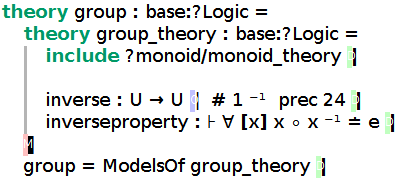
\includegraphics[width=8cm]{../MACIS17-interop/mitm1}}
  \caption{A Formalization of a Group}\label{fig:mitm1}
\end{figure}

At the representation level groups are described as concrete objects
suitable for computations: groups of permutations, groups of matrices,
finitely presented groups, groups obtained by algebraic constructions or using
polycyclic presentations.

At the implementation level, we encode implementation details: for
example, permutation groups are considered as finite subgroups of the group $S_{\mathbb{N}+}$, and defined \ednote{constructed?} by
providing a set of generating permutations.

At the concrete level, the computation happens: while the higher levels
are suitable for mathematical deduction and inference, this level is where OpenDreamKit systems like \GAP perform their main work.

\subsubsection{Modeling and Simulation}

The \href{https://gl.mathhub.info/MitM/smglom}{\texttt{models}}
archive (11 files, 650 LoF, 113 commits) is an experimental extension
of the MitM ontology, where we test the expressive power of MitM
framework (and the OpenDreamKit technologies) by applying it to a
field well outside of mathematics, namely for modeling and simulation
in opto-electronics.

\subsection{The ``Semantic Multilingual Glossary of Mathematics'' (SMGloM)}\label{sec:smglom}

The SMGloM library is available at \url{https://gl.mathhub.info/smglom}. It contains
ca. 815 glossary modules (OMDoc/MMT theories) with more than 1700 concepts. All
represented in \sTeX, a semantic variant of {\LaTeX} developed by FAU and (earlier at)
JacU. Figure~\ref{fig:conductor} shows an example. The boldface words are \emph{definienda}
(i.e. concepts to be defined; here ``conductor'') and the blue ones are concepts already
defined in other parts of the MitM Ontology. SMGloM definitions are multilingual -- mostly
English and German, but also some Romanian, Turkish, Arabic, and Chinese, and are
cross-linked on the concept level.

\ednote{specify what part of it was implemented in and out of \ODK}

\begin{figure}[ht]\centering
  \fbox{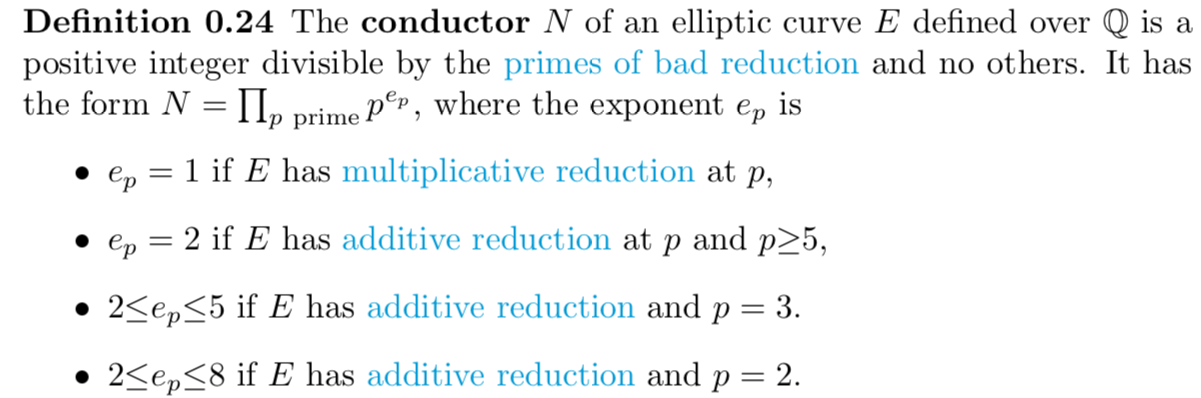
\includegraphics[width=14cm]{conductor}}
  \caption{An \sTeX Definition of the Conductor of an Elliptic
    Curve}\label{fig:conductor}
\end{figure}


%%% Local Variables:
%%% mode: visual-line
%%% fill-column: 5000
%%% mode: latex
%%% TeX-master: "report"
%%% End:

%  LocalWords:  formalizations texttt formalization standardization subsubsection textbf newcommand subseteq textsf MueRabKoh:tat18
%  LocalWords:  compactitem ednote adic ldots,a_n ldots,a_n ldots,T_n ldots Vec monoid sq
%  LocalWords:  FiniteHybridset subtyping emph leq_T leq_ leq_ leq_ r,x s,y leq doteq_T
%  LocalWords:  t,t forall subformula u,p ldots,x cdot cdot Qsqrt Qzeta th smglom fbox
%  LocalWords:  stabilizes fig:cgtontology fig:mitm1 centering includegraphics mathbb


% % % % % % % % % % % % % % % % % % % % % % % % % % % % % % % % % % % % %
\section{The ``Semantic Multilingual Glossary of Mathematics'' (SMGloM)}\label{sec:smglom}

The SMGloM library is available at \url{https://gl.mathhub.info/smglom}. It contains
ca. 815 glossary modules (OMDoc/MMT theories) with more than 1700 concepts. All
represented in \sTeX, a semantic variant of {\LaTeX} developed by FAU and (earlier at)
JacU. Figure~\ref{fig:conductor} shows an example. The boldface words are \emph{definienda}
(i.e. concepts to be defined; here ``conductor'') and the blue ones are concepts already
defined in other parts of the MitM Ontology. SMGloM definitions are multilingual -- mostly
English and German, but also some Romanian, Turkish, Arabic, and Chinese, and are
cross-linked on the concept level.

\ednote{specify what part of it was implemented in and out of \ODK}

\begin{figure}[ht]\centering
  \fbox{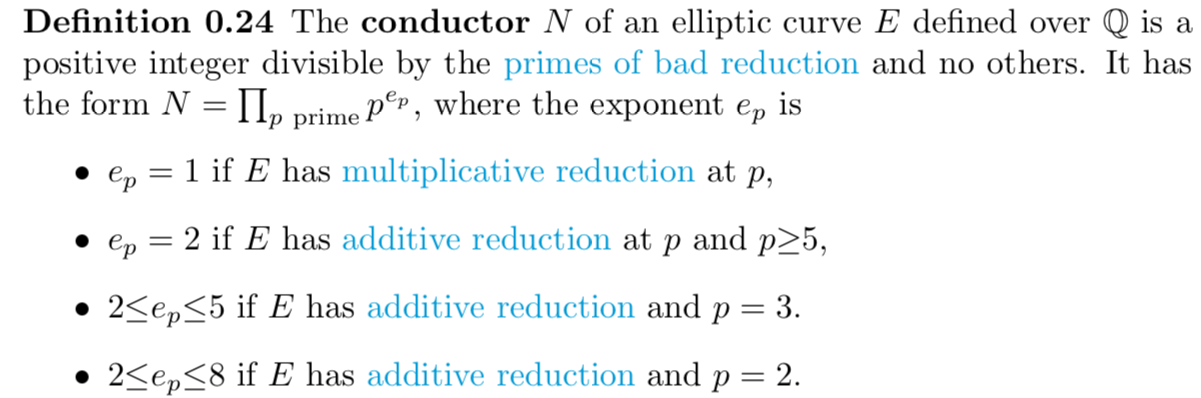
\includegraphics[width=14cm]{conductor}}
  \caption{An \sTeX Definition of the Conductor of an Elliptic
    Curve}\label{fig:conductor}
\end{figure}

\subsection{The OpenDreamKit System APIs}\label{sec:sysapis}

We have generated and cross-linked system APIs for the computer algebra systems GAP,
SageMath, and SINGUALAR, they can be found at
\url{https://gl.mathhub.info/ODK/{GAP,SAGE,SINGULAR,LMFDB}}.\ednote{MK: write some more}

\subsection{The MitM Alignments}

The MitM alignments are available from \url{https://gl.mathhub.info/alignments/Public} (6
files, 1040 LoF, 240 Commits). They are represented as text files containing pairs of MMT
URIs annotated with various semantic classification schemata;
see~\cite{MueGauKal:cacfms17} for details.\ednote{MK: what else can we write about them?}
\ednote{this figure does not fit in the text width}
\begin{figure}[ht]\centering
  \tikzinput[width=.98\textwidth]{../D6.5/alignmentimg}
  \caption{Alignments between the MitM Ontology and the \GAP API}\label{fig:cgtontology}
\end{figure}

As an example, Figure~\ref{fig:cgtontology} sketches the alignments between the
computational group theory ontology from above and the constructors and operations of
\GAP.

\section{Evaluation \& Conclusion}\label{sec:concl}

Figure~\ref{fig:MitM-graph} shows an overview of the MitM ontology, together with the
system APIs and the alignments (in red). We can directly see that the MitM ontology is
dwarfed by the system API graphs. This is to be expected, since we have mainly covered the
background knowledge needed for the OpenDreamKit integration use cases;
see~\cite{ODK-D6.5}. This is in sync with the overall project plan, which mainly wants to
demonstrate the feasibility of the MitM approach to system integration, and expects the
main part of the MitM Ontology to be contributed by the mathematical community.

Most of the work in MitM Ontology has gone into provisioning a viable foundation
and basic set of types, which allow the flexiformalization and specification of
mathematical knowledge, objects, functions, and types in a system-independent/neutral way
that closely mirrors the presentation in the mathematical literature. The central focus
was in the naturalness and adequacy of the representation. The focus on a basic repertoire
of types inspired by mathematical practice goes a long way into this direction.

With CGT (computational group theory) we have shown that the MitM approach is feasible,
and that the investment into the extension of the MitM Ontology is commensurate with
writing good (mathematical) documentation. Indeed the MitM ontology together with the
system API alignments can be used for documentation purposes and complement it. Moreover, as
MitM representations are shared between systems by design, all systems participating in
the OpenDreamKit MitM-based integration scheme obtain this ``documentation'' for the cost
of alignments alone. 

Generally, we note that the investment necessary for adding mathematical functionality to
the MitM integration decreases with the size of the existing MitM ontology, and in the
limit becomes proportional to the size of the added functionality, while the amount of
system functionality yielded by MitM-compatible systems increases proportionally with the
MitM size. Already with four systems GAP, Sage, Singular, and LMFDB; see~\cite{ODK-D6.5}
we have reached a size where investments into extending the MitM ontology are starting to
pay off, and interest of the computational mathematics is generated. We expect that, once
the heavy lifting of getting the framework and a seed MitM Ontology has been done,
the integration framework and MitM Ontology coverage will grow organically.

\begin{figure}\centering
  \fbox{\begin{sideways}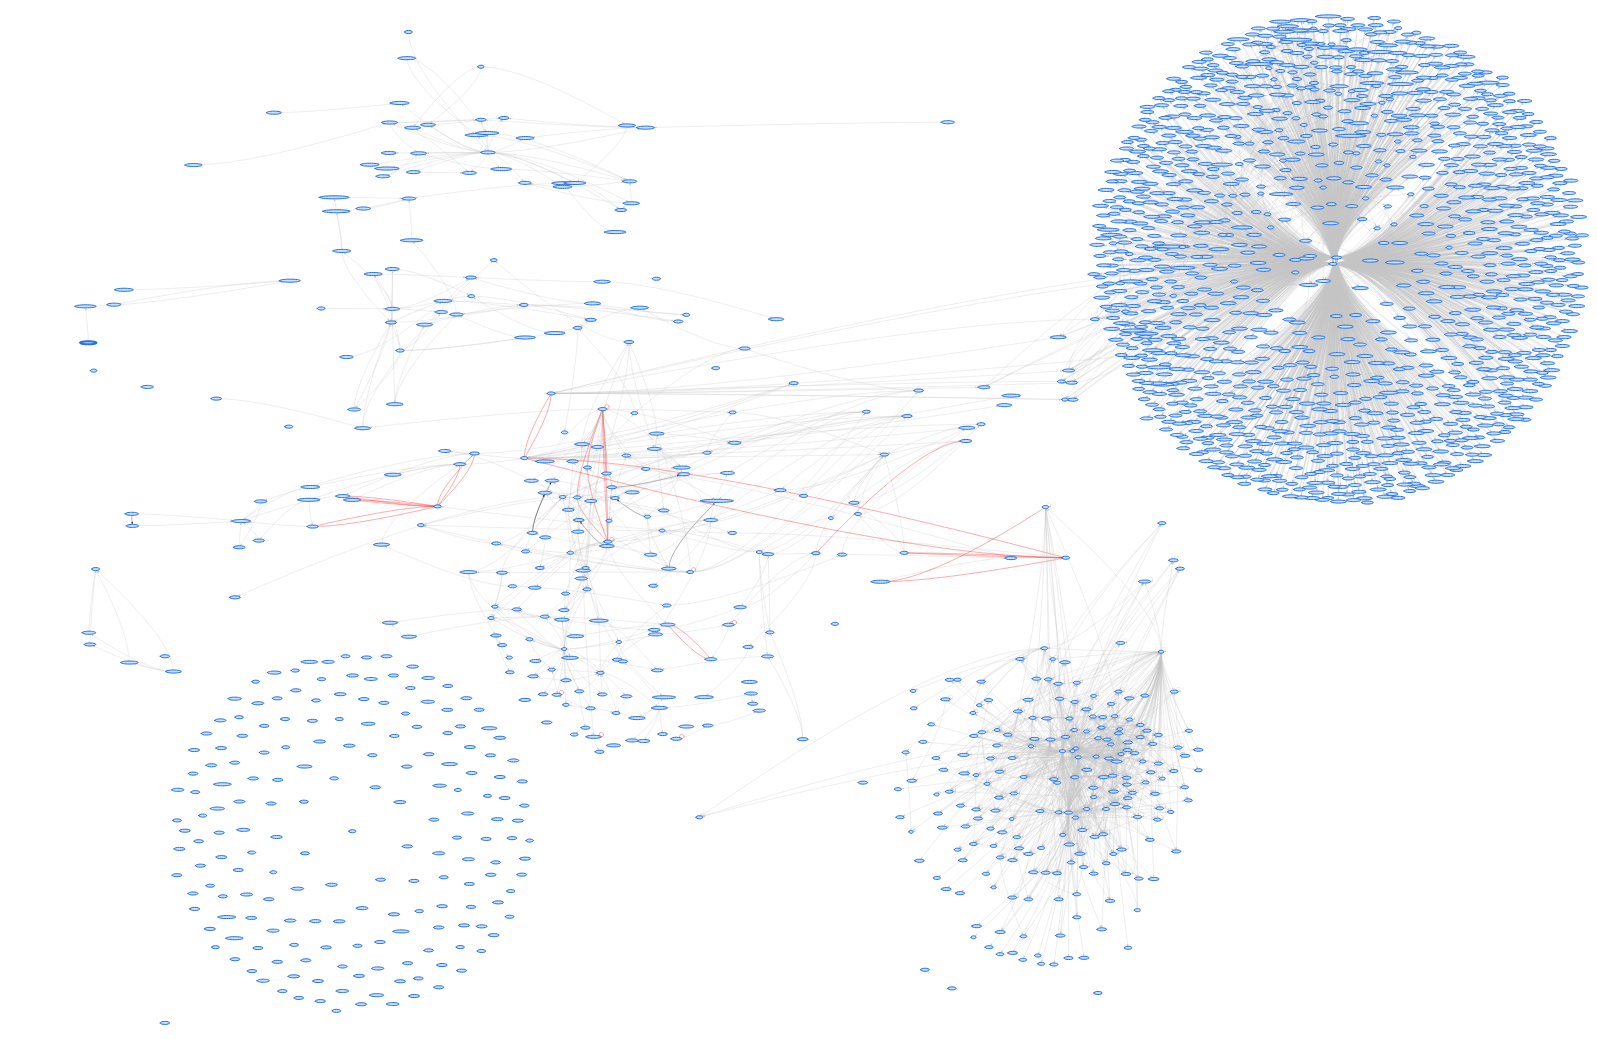
\includegraphics[width=.95\textheight]{MitM-graph}\end{sideways}}
%  \fbox{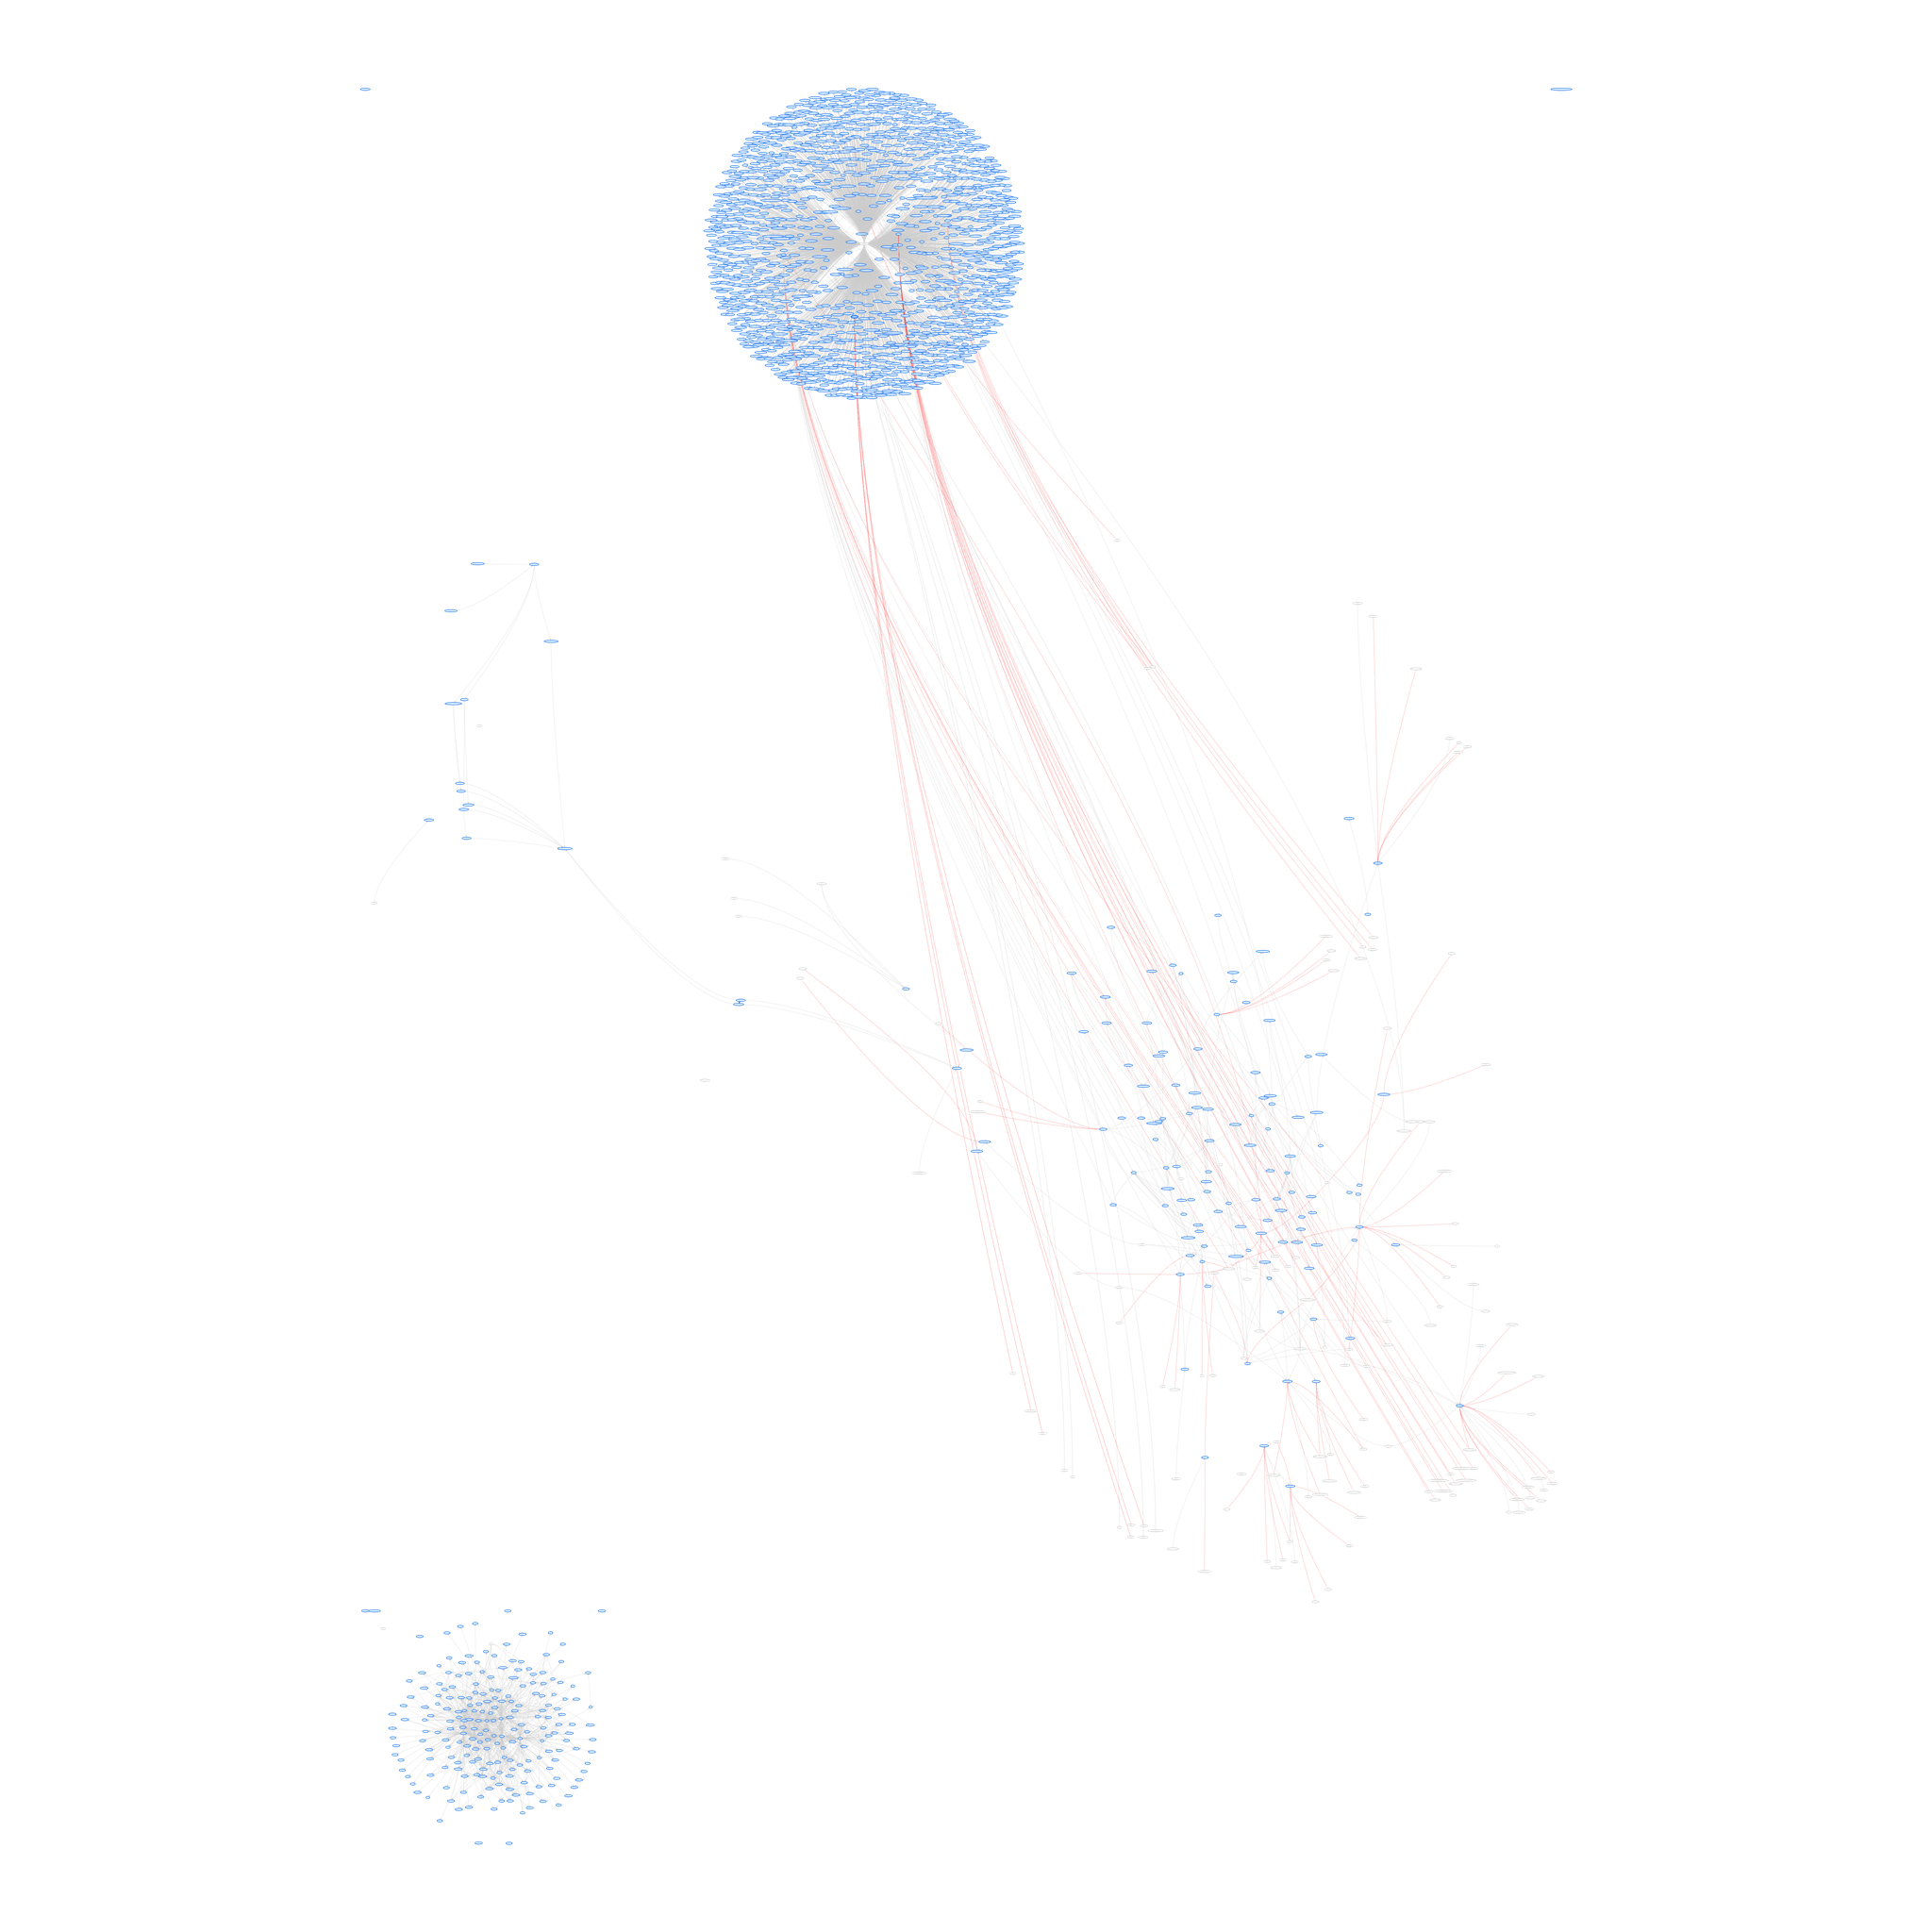
\includegraphics[width=.95\textwidth]{MitM-graph1}}
  \caption{The MitM Theory Graph}\label{fig:MitM-graph}
\end{figure}

\newpage\printbibliography\newpage

\begin{appendix}
  \section{Types}\label{app:types}

Based on a survey of the OpenDreamKit systems, we have identified the following types for the MitM Foundation (see Section \ref{sec:foundation}); see Appendix~\ref{app:expr} for an exemplary list of mathematical objects that can be represented as a members of these types.

\subsection{Base Types}
\begin{compactitem}
 \item number types (all unbounded in size):
  \begin{compactitem}
   \item natural numbers: $N$ (including $0$), $Pos$ (positive, excluding $0$), $Prime$ (prime numbers, not excluding $0$ and $1$)
   \item integer numbers: $Z$
   \item integer numbers modulo $m$: $Z(m)$ (for $m\in Pos$)
   \item rational numbers: $Q$
   \item real numbers: $R$ \ednote{FR: it's unclear which irrational numbers we need to support and how to represent them}
   \item complex numbers: $C$
   \item $p$-adic numbers: $Qp(p)$ (for prime $p$)
  \end{compactitem}
 \item strings: $String$
 \item booleans: $Boolean$
 \end{compactitem}

 \subsection{Complex Types}
 \begin{itemize}
\item Function types
 \begin{itemize}
 \item the type $T_1\to T_2$ of total functions from $T_1$ to $T_2$,
 \item shallow polymorphic types $\{a_1,\ldots,a_n\}T(a_1,\ldots,a_n)$ for a type $T$ with $n$ free type variables, with the restriction that polymorphic types may not occur as subexpressions of any of the other type constructors,
 \end{itemize}
\item Aggregating type constructors for types $T_1,\ldots,T_n$
\begin{compactitem}
 \item product types: $T_1*\cdots * T_n$
 \item record types: $\record{a_1: T_1, \ldots, a_n:T_n}$ for identifiers $a_i$
 \item disjoint union types: $T_1+\ldots + T_n$ \ednote{FR: not sure if we need these as they rarely come up yet as they are dual to product types}
 \item labeled disjoint union types: $\union{a_1:T_1,\ldots,a_n: T_n}$ for identifiers $a_i$ \ednote{FR: not sure if we need these as they rarely come up yet; they are dual to record types}
\end{compactitem}
In record and labeled disjoint union types, the order of fields is not relevant.
\item Collecting type constructors for any type $T$
\begin{compactitem}
 \item option types (list of length up to $1$): $Opt(T)$
 \item vectors (fixed-length lists): $Vec(T,n)$ for $n\in N$
 \item lists (arbitrary finite length): $List(T)$
 \item sets (finite subsets): $FiniteSet(T)$
 \item multisets (finite multiset subsets): $FiniteMultiset(T)$
 \item finite hybrid sets: $FiniteHybridset(T)$ are like multisets but also allow negative
   multiplicities.
 \item matrices: $Mat(T,m,n)$ for $m,n\in N$
\end{compactitem}
\item Erasure of dependent parameters: for a type constructor $T(k)$ (not necessarily unary) that takes a parameter $k$ of number type, we write $T(\_)$ for the type obtained by taking the unions over all possible parameters. In particular, we have
\begin{compactitem}
 \item $Mat(T,m,\_)$, $Mat(T,\_,n)$ and $Mat(T,\_,\_)$ for matrices with arbitrary dimensions
 \item $List(T)=Vec(T,\_)$
 \end{compactitem}
\end{itemize}

\subsection{Types for Mathematical Structures and their Models}

\begin{compactitem}
 \item finite maps (partial functions with finite support): $FiniteMap(T_1,T_2)$ for types $T_i$
 \item polynomials: $Polynomial(r,[x_1,\ldots x_n])$ for ring $r\in Ring$ and identifiers $x_i$
 \item rings: $Ring$ (multiplication is a commutative monoid)
 \item fields: $Field$
 \item elements of structures: every structure $S$ (e.g., $S\in Ring$ or $S\in Field$) is a type itself; the elements of $S$ are represented as elements of the underlying type of $S$, which must be defined separately for every structure $S$.
\end{compactitem}
More generally than fixing $Ring$ and $Field$, we actually allow $Mod(T)$ for any theory $T$.
But the types listed above are sufficient for our purposes here.

\subsection{Subtyping}

The \textbf{subtyping} relation $S\sq T$ is the order generated by
\begin{compactitem}
 \item $Prime\sq Pos\sq N\sq Z\sq Q\sq R\sq C$
 \item $T(k)\sq T(\_)$ for any type constructor $T$ (not necessarily unary) that allows a wildcard parameter
 \item All collecting and aggregating type constructors are covariant in all type arguments. For example, if $S\sq T$, then $List(S)\sq List(T)$.
 \item Horizontal subtyping: Record types become smaller, labeled disjoint union types bigger when adding fields.
 \item $FiniteMap$ is covariant in both type arguments.\footnote{Note that it is normal for \emph{partial} functions to be covariant in the domain.}
 \item $Ring\sq Field$
 \item For structures $s,S$ of type $T$, we have $s\sq S$ iff $s\leq_T S$. 
\end{compactitem}

Here we have used the submodel order $s\leq_T S$ which holds if $s$ is submodel of $S$ with respect to theory $T$.
$T$ can be the type of models of any theory, but for our purposes, it is sufficient to consider only the case $T\in\{Ring,Field\}$.
We use only the following sub-models
\begin{compactitem}
 \item $Z\leq_{Ring} Q\leq_{Field} R\sq\leq_{Field} C$
 \item $Polynomial(r,x)\leq_{Ring} Polynomial(s,y)$ if $r\leq_{Ring} s$ and every variable in $x$ also occurs in $y$.
 \item If $T\sq T'$, then $s\leq_T S$ implies $s\leq{T'}S$.
\end{compactitem}


%%% Local Variables:
%%% mode: latex
%%% mode: visual-line
%%% fill-column: 5000
%%% TeX-master: "report"
%%% End:

\end{appendix}
\end{document}

%%% Local Variables:
%%% mode: visual-line
%%% fill-column: 5000
%%% mode: latex 
%%% TeX-master: t
%%% End:

%  LocalWords:  maketitle newpage tableofcontents newpage newcommand xspace ednote mathdb
%  LocalWords:  standardize dktheories concl printbibliography pn textit mmt mitm emph
%  LocalWords:  WPref dksbases prioritized taskref organized delivref dkstheories textbf
%  LocalWords:  githubissuedescription MueGauKal:cacfms17 MueRoYuRa:abtafs17 compactenum
%  LocalWords:  DehKohKon:iop16,WieKohRab:vtuimkb17,KohMuePfe:kbimss17 formalization fbox
%  LocalWords:  texttt subtyping flexary smglom stabilizes formalizations centering
%  LocalWords:  includegraphics fig:condutor textheight fig:cgtontology textwidth
%  LocalWords:  alignmentimg flexiformalization sec:mitmonto tikzinput
